\documentclass{standalone}
\usepackage{tikz}
\usetikzlibrary{patterns, positioning}

\begin{document}
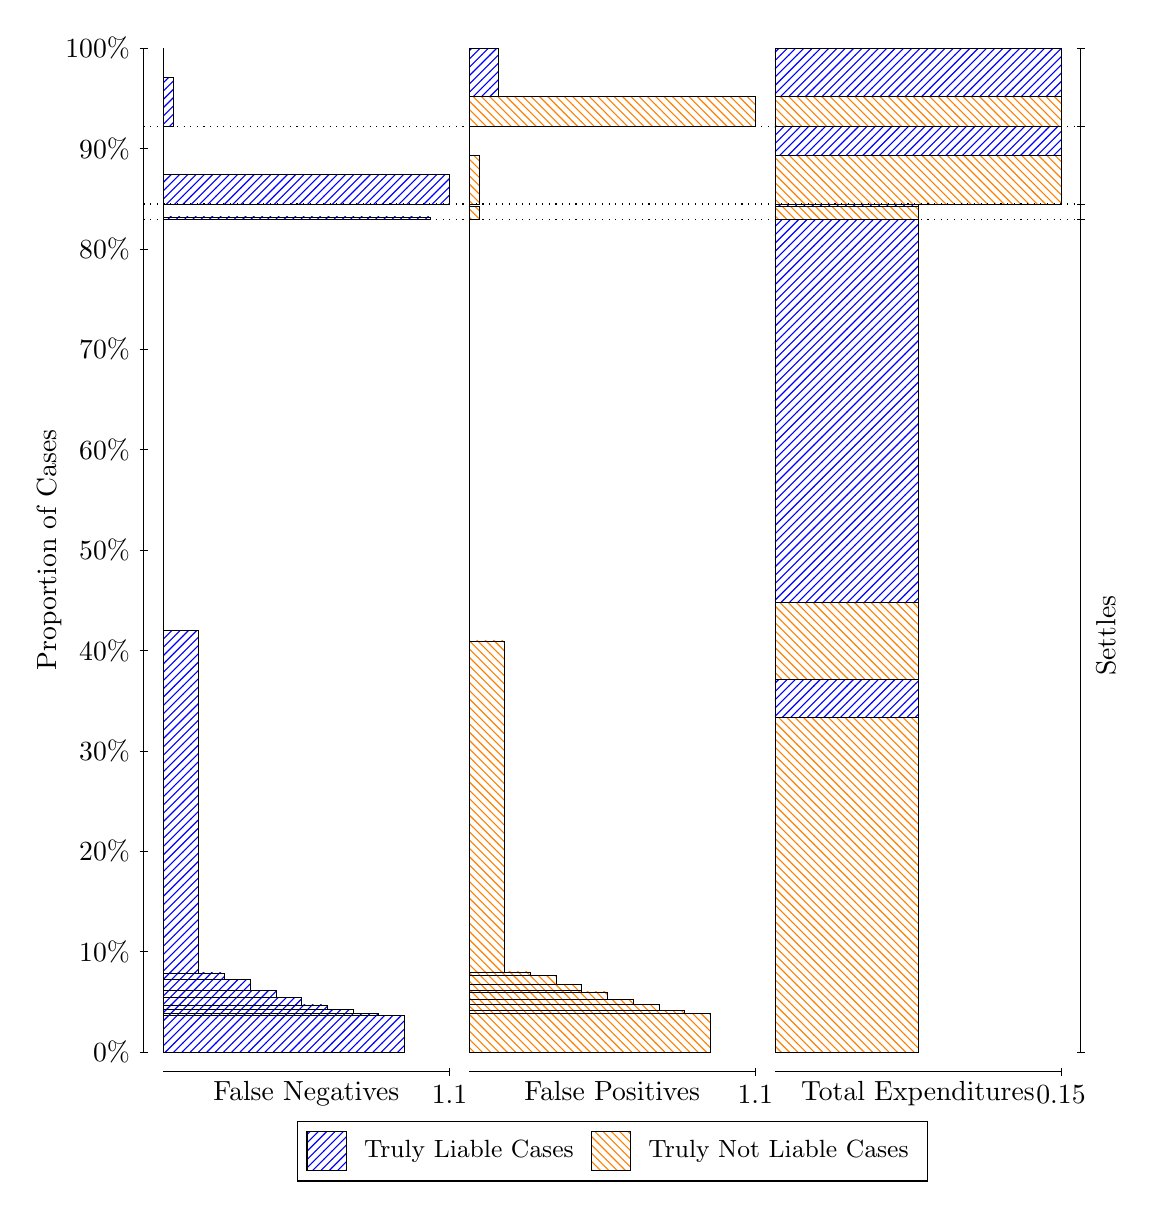
\begin{tikzpicture}
\draw[black, very thin] (1.5,1.75) -- (1.5,14.5);
\node[rotate=90, anchor=center] at (0.3, 8.125) {Proportion of Cases};
\draw[black, very thin] (1.45,1.75) -- (1.55,1.75);
\node[anchor=east] at (1.45, 1.75) {0\%};
\draw[black, very thin] (1.45,3.025) -- (1.55,3.025);
\node[anchor=east] at (1.45, 3.025) {10\%};
\draw[black, very thin] (1.45,4.3) -- (1.55,4.3);
\node[anchor=east] at (1.45, 4.3) {20\%};
\draw[black, very thin] (1.45,5.575) -- (1.55,5.575);
\node[anchor=east] at (1.45, 5.575) {30\%};
\draw[black, very thin] (1.45,6.85) -- (1.55,6.85);
\node[anchor=east] at (1.45, 6.85) {40\%};
\draw[black, very thin] (1.45,8.125) -- (1.55,8.125);
\node[anchor=east] at (1.45, 8.125) {50\%};
\draw[black, very thin] (1.45,9.4) -- (1.55,9.4);
\node[anchor=east] at (1.45, 9.4) {60\%};
\draw[black, very thin] (1.45,10.675) -- (1.55,10.675);
\node[anchor=east] at (1.45, 10.675) {70\%};
\draw[black, very thin] (1.45,11.95) -- (1.55,11.95);
\node[anchor=east] at (1.45, 11.95) {80\%};
\draw[black, very thin] (1.45,13.225) -- (1.55,13.225);
\node[anchor=east] at (1.45, 13.225) {90\%};
\draw[black, very thin] (1.45,14.5) -- (1.55,14.5);
\node[anchor=east] at (1.45, 14.5) {100\%};

\draw[black, very thin] (13.4,1.75) -- (13.4,14.5);
\draw[black, very thin] (13.35,1.75) -- (13.45,1.75);
\node[anchor=west] at (13.35, 1.75) {};
\draw[black, very thin] (13.35,12.322) -- (13.45,12.322);
\node[anchor=west] at (13.35, 12.322) {};
\draw[black, very thin] (13.35,12.519) -- (13.45,12.519);
\node[anchor=west] at (13.35, 12.519) {};
\draw[black, very thin] (13.35,13.509) -- (13.45,13.509);
\node[anchor=west] at (13.35, 13.509) {};
\draw[black, very thin] (13.35,14.5) -- (13.45,14.5);
\node[anchor=west] at (13.35, 14.5) {};

\draw[black, very thin, pattern color=blue, pattern=north east lines] (1.75,1.75) rectangle (4.8118,2.218);
\draw[black, very thin, pattern color=blue, pattern=north east lines] (1.75,2.218) rectangle (4.4852,2.2381);
\draw[black, very thin, pattern color=blue, pattern=north east lines] (1.75,2.2381) rectangle (4.1586,2.2949);
\draw[black, very thin, pattern color=blue, pattern=north east lines] (1.75,2.2949) rectangle (3.832,2.3478);
\draw[black, very thin, pattern color=blue, pattern=north east lines] (1.75,2.3478) rectangle (3.5054,2.4437);
\draw[black, very thin, pattern color=blue, pattern=north east lines] (1.75,2.4437) rectangle (3.1788,2.5293);
\draw[black, very thin, pattern color=blue, pattern=north east lines] (1.75,2.5293) rectangle (2.8522,2.6754);
\draw[black, very thin, pattern color=blue, pattern=north east lines] (1.75,2.6754) rectangle (2.5257,2.7539);
\draw[black, very thin, pattern color=blue, pattern=north east lines] (1.75,2.7539) rectangle (2.1991,7.101);
\draw[black, very thin, pattern color=orange, pattern=north west lines] (1.75,7.101) rectangle (1.75,12.322);
\draw[black, very thin, pattern color=blue, pattern=north east lines] (1.75,12.322) rectangle (5.1384,12.355);
\draw[black, very thin, pattern color=orange, pattern=north west lines] (1.75,12.355) rectangle (1.75,12.519);
\draw[black, very thin, pattern color=blue, pattern=north east lines] (1.75,12.519) rectangle (5.3833,12.896);
\draw[black, very thin, pattern color=orange, pattern=north west lines] (1.75,12.896) rectangle (1.75,13.509);
\draw[black, very thin, pattern color=blue, pattern=north east lines] (1.75,13.509) rectangle (1.8725,14.123);
\draw[black, very thin, pattern color=orange, pattern=north west lines] (1.75,14.123) rectangle (1.75,14.5);
\draw[black, very thin, pattern color=orange, pattern=north west lines] (5.6333,1.75) rectangle (8.6951,2.243);
\draw[black, very thin, pattern color=orange, pattern=north west lines] (5.6333,2.243) rectangle (8.3685,2.278);
\draw[black, very thin, pattern color=orange, pattern=north west lines] (5.6333,2.278) rectangle (8.0419,2.3558);
\draw[black, very thin, pattern color=orange, pattern=north west lines] (5.6333,2.3558) rectangle (7.7154,2.4141);
\draw[black, very thin, pattern color=orange, pattern=north west lines] (5.6333,2.4141) rectangle (7.3888,2.5118);
\draw[black, very thin, pattern color=orange, pattern=north west lines] (5.6333,2.5118) rectangle (7.0622,2.5356);
\draw[black, very thin, pattern color=orange, pattern=north west lines] (5.6333,2.5356) rectangle (7.0622,2.6046);
\draw[black, very thin, pattern color=orange, pattern=north west lines] (5.6333,2.6046) rectangle (6.7356,2.7224);
\draw[black, very thin, pattern color=orange, pattern=north west lines] (5.6333,2.7224) rectangle (6.409,2.7682);
\draw[black, very thin, pattern color=orange, pattern=north west lines] (5.6333,2.7682) rectangle (6.0824,6.9706);
\draw[black, very thin, pattern color=blue, pattern=north east lines] (5.6333,6.9706) rectangle (5.6333,12.322);
\draw[black, very thin, pattern color=orange, pattern=north west lines] (5.6333,12.322) rectangle (5.7558,12.485);
\draw[black, very thin, pattern color=blue, pattern=north east lines] (5.6333,12.485) rectangle (5.6333,12.519);
\draw[black, very thin, pattern color=orange, pattern=north west lines] (5.6333,12.519) rectangle (5.7558,13.132);
\draw[black, very thin, pattern color=blue, pattern=north east lines] (5.6333,13.132) rectangle (5.6333,13.509);
\draw[black, very thin, pattern color=orange, pattern=north west lines] (5.6333,13.509) rectangle (9.2667,13.886);
\draw[black, very thin, pattern color=blue, pattern=north east lines] (5.6333,13.886) rectangle (6.0007,14.5);
\draw[black, very thin, pattern color=orange, pattern=north west lines] (9.5167,1.75) rectangle (11.333,5.9983);
\draw[black, very thin, pattern color=blue, pattern=north east lines] (9.5167,5.9983) rectangle (11.333,6.4863);
\draw[black, very thin, pattern color=orange, pattern=north west lines] (9.5167,6.4863) rectangle (11.333,7.4587);
\draw[black, very thin, pattern color=blue, pattern=north east lines] (9.5167,7.4587) rectangle (11.333,12.322);
\draw[black, very thin, pattern color=orange, pattern=north west lines] (9.5167,12.322) rectangle (11.333,12.485);
\draw[black, very thin, pattern color=blue, pattern=north east lines] (9.5167,12.485) rectangle (11.333,12.519);
\draw[black, very thin, pattern color=orange, pattern=north west lines] (9.5167,12.519) rectangle (13.15,13.132);
\draw[black, very thin, pattern color=blue, pattern=north east lines] (9.5167,13.132) rectangle (13.15,13.509);
\draw[black, very thin, pattern color=orange, pattern=north west lines] (9.5167,13.509) rectangle (13.15,13.886);
\draw[black, very thin, pattern color=blue, pattern=north east lines] (9.5167,13.886) rectangle (13.15,14.5);
\draw[black, dotted] (1.5,12.322) -- (13.4,12.322);
\draw[black, dotted] (1.5,12.519) -- (13.4,12.519);
\draw[black, dotted] (1.5,13.509) -- (13.4,13.509);
\draw[black, very thin] (1.75,1.5) -- (5.3833,1.5);
\node[anchor=north] at (3.5667, 1.5) {False Negatives};
\draw[black, very thin] (5.3833,1.45) -- (5.3833,1.55);
\node[anchor=north] at (5.3833, 1.45) {1.1};

\draw[black, very thin] (5.6333,1.5) -- (9.2667,1.5);
\node[anchor=north] at (7.45, 1.5) {False Positives};
\draw[black, very thin] (9.2667,1.45) -- (9.2667,1.55);
\node[anchor=north] at (9.2667, 1.45) {1.1};

\draw[black, very thin] (9.5167,1.5) -- (13.15,1.5);
\node[anchor=north] at (11.333, 1.5) {Total Expenditures};
\draw[black, very thin] (13.15,1.45) -- (13.15,1.55);
\node[anchor=north] at (13.15, 1.45) {0.15};

\node[black, centered, rotate=90] at (13.72, 7.0358) {Settles};




\draw (7.449999999999999,1.5) node[draw=none] (baseCoordinate) {};
\begin{scope}[align=center]
        \matrix[scale=0.5, draw=black, below=0.5cm of baseCoordinate, nodes={draw}, column sep=0.1cm]{
            \node[rectangle, draw, minimum width=0.5cm, minimum height=0.5cm, pattern=north east lines, pattern color=blue] {}; &
            \node[draw=none, font=\small] (B) {Truly Liable Cases}; &
            \node[rectangle, draw, minimum width=0.5cm, minimum height=0.5cm, pattern=north west lines, pattern color=orange] {}; &
            \node[draw=none, font=\small] (B) {Truly Not Liable Cases}; \\
            };
\end{scope}

\end{tikzpicture}
\end{document}